% Standalone vector artwork. Build with xelatex trial-designs.tex.
% EPS conversion: pdftops -eps -level3 trial-designs.pdf trial-designs.eps
\documentclass[tikz,border=2.5pt]{standalone}
\usepackage[no-math]{fontspec}
\setsansfont[Scale=.94]{Arial}
\usetikzlibrary{arrows.meta}
\definecolor{ink}{HTML}{27323B}
\definecolor{stroke}{HTML}{586470}
\definecolor{treated}{HTML}{236540}
\definecolor{internal}{HTML}{305F90}
\definecolor{external}{HTML}{72488C}
\definecolor{lightgreen}{HTML}{E9F3EC}
\definecolor{lightblue}{HTML}{E9F0F9}
\definecolor{lightpurple}{HTML}{F2EDF7}
\begin{document}
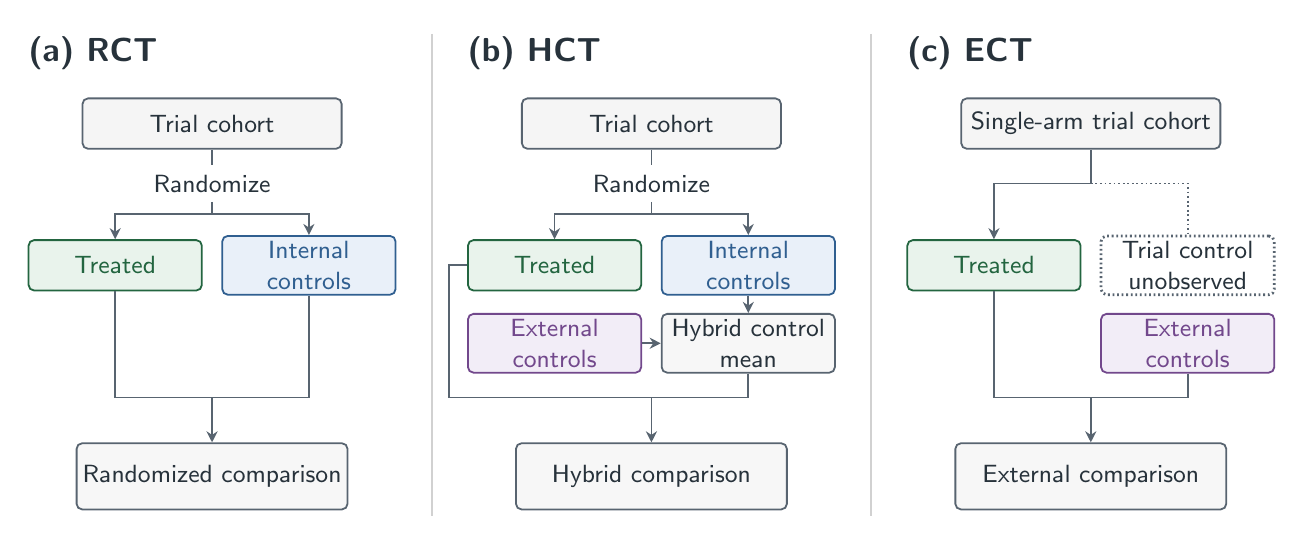
\begin{tikzpicture}[
 x=1cm,y=1cm,font=\sffamily\fontsize{9.5}{11}\selectfont,text=ink,
 group/.style={draw=stroke,line width=.65pt,rounded corners=2pt,
               align=center,inner sep=2pt,minimum height=.64cm},
 cohort/.style={group,fill=black!4,text width=3.15cm},
 treat/.style={group,draw=treated,fill=lightgreen,text=treated,text width=2.06cm},
 ic/.style={group,draw=internal,fill=lightblue,text=internal,text width=2.06cm},
 ec/.style={group,draw=external,fill=lightpurple,text=external,text width=2.06cm},
 missing/.style={group,draw=stroke,densely dotted,line width=1pt,text width=2.06cm},
 endpoint/.style={group,minimum height=.69cm,text width=3.30cm},
 title/.style={anchor=west,inner xsep=0pt,font=\sffamily\bfseries\fontsize{12}{14}\selectfont},
 line/.style={draw=stroke,line width=.65pt},
 arrow/.style={line,-{Stealth[length=4pt,width=4pt]}}]
\newcommand{\randomarms}{%
  \node[cohort] (trial) at (0,0) {Trial cohort};
  \node[align=center] (random) at (0,-.76) {Randomize};
  \draw[line] (trial.south) -- (random.north);
  \node[treat] (t) at (-1.23,-1.80) {Treated};
  \node[ic] (c) at (1.23,-1.80) {Internal controls};
  \draw[line] (random.south) -- (0,-1.15);
  \draw[arrow] (0,-1.15) -| (t.north);
  \draw[arrow] (0,-1.15) -| (c.north);
}
% Connect two observed groups to the common contrast. Both connections enter
% after treatment assignment; neither assigns treatment to an external record.
\newcommand{\compare}[1]{%
  \node[endpoint,fill=black!3,minimum height=.84cm] (comp) at (0,-4.48) {#1};
  \draw[line] (l.south) -- (l.south |- 0,-3.48) -- (0,-3.48);
  \draw[line] (r.south) -- (r.south |- 0,-3.48) -- (0,-3.48);
  \draw[arrow] (0,-3.48) -- (comp.north);
}
\begin{scope}
  \node[title] at (-2.34,.89) {(a) RCT};
  \randomarms
  \coordinate (l) at (t.south); \coordinate (r) at (c.south);
  \compare{Randomized comparison}
\end{scope}
\draw[black!18,line width=.6pt] (2.79,1.14) -- (2.79,-4.98);
\begin{scope}[xshift=5.58cm]
  \node[title] at (-2.34,.89) {(b) HCT};
  \randomarms
  \node[ec] (extern) at (-1.23,-2.79) {External controls};
  \node[group,fill=black!3,text width=2.06cm] (aug) at (1.23,-2.79) {Hybrid control\\mean};
  \draw[arrow] (c.south) -- (aug.north);
  \draw[arrow] (extern.east) -- (aug.west);
  \node[endpoint,fill=black!3,minimum height=.84cm] (comp) at (0,-4.48) {Hybrid comparison};
  \draw[line] (t.west) -- (-2.57,-1.80) -- (-2.57,-3.48) -- (0,-3.48);
  \draw[line] (aug.south) -- (1.23,-3.48) -- (0,-3.48);
  \draw[arrow] (0,-3.48) -- (comp.north);
\end{scope}
\draw[black!18,line width=.6pt] (8.37,1.14) -- (8.37,-4.98);
\begin{scope}[xshift=11.16cm]
  \node[title] at (-2.34,.89) {(c) ECT};
  \node[cohort] (trial) at (0,0) {Single-arm trial cohort};
  \node[treat] (t) at (-1.23,-1.80) {Treated};
  \node[missing] (counter) at (1.23,-1.80) {Trial control\\unobserved};
  \draw[arrow] (trial.south) -- (0,-.76) -| (t.north);
  \draw[line,densely dotted] (0,-.76) -| (counter.north);
  \node[ec] (extern) at (1.23,-2.79) {External controls};
  \coordinate (l) at (t.south); \coordinate (r) at (extern.south);
  \compare{External comparison}
\end{scope}
\end{tikzpicture}
\end{document}
